\section{Integration of ACES into rVBQC}
% \todo[holl,inline]{
% \\- Traps are sensitive to errors as they are detecting deviations
% \\- They get information about the errors happening on neighboring qubits. Depending on the error model this can be a gate that touches the trap qubit or one of its neighbor. Or further apart in case of cross-talk.
% \\- The value of the trap is given by an ACES-like equation.
% \\- The fundamental difference is we cannot vary the circuit beyond the order of the gates
% \\- In the simplest model there is no possibility to infer the noise parameters without varying the order
% \\- Main question is how to infer this?}
In this section, we show how ACES can be integrated into rVBQC. To this end, we will proceed in 3 steps: first, we review briefly rVBQC and its security guarantees; second, we show that some information about noise can be extracted by the protocol from the point of view of the server in a way that resembles ACES; third we show that, while the structural rigidity of rVBQC seems to jeopardize ACES, it is indeed possible to blend the two protocols into a new one that:
\begin{enumerate}
\item Achieves the same security and noise-robustness guarantees as the original rVBQC;
\item Allows the server to extract noise parameters for a wide variety of Pauli channels.
\end{enumerate}

\subsection{Verification and rVBQC}
\label{sec:verification}

The security guarantees of rVBQC are given in the Abstract Cryptography (AC) framework \cite{MR11abstract-cryptography}. This framework not only provides a general structure for security proofs, but most interestingly shows that whenever a protocol is secure in AC, then it is inherently composable. More concretely, this means that this protocol can be safely used within the context of a larger protocol without having to reprove its security in this new context. This contrasts with stand-alone security proofs whose security guarantees hold only in isolation.

The high-level methodology imposed by AC is to first define an ideal resource. It is nothing more than a mathematical specification of what the final device is supposed to do. For instance, when a client asks for verifying a computation \(\cptp{C}\) delegated to a server, this means that either it receives the correct result or it receives \(\Abort\). This means that it is never forced to accept an incorrect result. This is also the best that it can ask, as it cannot force the server to perform the computation, e.g., the server can always refuse to send the computation result. Additionally, rVBQC provides blindness, which means that the server ``does not know'' the computation \(C\) being delegated. Obviously, the server will still at least have an upper bound on the size of the computation simply because it can measure the time it takes per round. To encompass this unavoidable leakage of information, blindness will be relative to a set of computations \(\mathfrak{C}\) in the sense that while delegating \(\cptp{C}\in \mathfrak{C}\), the server learns at most \(\mathfrak{C}\).

All of this can now be summarized in the following Secure Delegated Quantum Computation resource:
\begin{resource}[Secure Delegated Quantum Computation]
  \label{res:sdqc}
  \item
  \begin{algorithmic}[0]
    \State \textbf{Public information}: Nature of the permitted leakage.
    \State \textbf{Permitted leakage}: Set of computations \(\mathfrak{C}\).
    \State \textbf{Client's input}: A classical description of \(\mathsf{C} \in \mathfrak{C}\).
    \State \textbf{Server's input}: Two bits \(c,d\).
    \Procedure{Resource's operations}{}
    \State It receives the client's input.
    \State If it receives \(c=1\), it sends the leakage to the server who returns \(d\).
    \State If \(d=1\), it outputs \(\Abort\) at the client's interface.
    \State If \(c=0\) or \(c=1 \wedge d=0\), it outputs the result of computation \(\mathsf{C}\) and \(\Acc\) at the client's interface.
    \EndProcedure
  \end{algorithmic}
\end{resource}
This resource is deemed \emph{secure-by-design} because it is the transcription of the input-output relationships that can be deduced from the plain-English description of the functionality it corresponds to. 

In particular, AC specifies that the definition of an ideal resource does not propose an implementation. The implementation is actually the second step in the AC methodology and corresponds to the protocol. For rVBQC, it works in the following way:
\begin{protocol}[rVBQC]
\label{proto:rvbqc}
\item
  \begin{algorithmic}[0]
    \State \textbf{Public information}: 
    \begin{itemize}
    \item A graph \(G\) and a flow \(f\).
    \item Integers \(N,d,w\) with \(d < N\) and \(w  < N-d\) representing the total number of rounds, the number of computation rounds, and the number of tolerated failed test rounds.
    \end{itemize}
    \State \textbf{Client's input}: \(P\), a MBQC pattern over \(G\) and compatible with the flow \(f\).
    \State The client samples the location of \(d\) computation rounds in \([N]\).
    \Procedure{Round Delegation}{}
    \State If the round is a computation round, prepare all qubits in \(\ket+\) and delegate the MBQC pattern \(P\) to the server using UBQC (\cref{proto:ubqc}).
    \State If the round is a test round, perform the qubit preparation and obtain the MBQC pattern \(T\) using \cref{routine:test-sampling}, then delegate it to the server using UBQC (\cref{proto:ubqc}), both detailed in \cref{sec:ubqc}.
    \EndProcedure
    \Procedure{Deviation detection}{}
    \State The client counts the number of failed test rounds (i.e., rounds for which at least one of the trap measurements does not correspond to a +1 outcome).
  \State If the number of failed test rounds is greater than \(w\), output \(\Abort\).
  \EndProcedure
  \Procedure{Majority vote}{}
  \State If the protocol has not aborted, compute the majority vote of the results of computation rounds and output it together with \(\Acc\).
  \EndProcedure
  \end{algorithmic}
\end{protocol}
First, note that the set of computations  \(\mathfrak{C}\) for which the protocol is blind is relative to all computations that can be performed using a graph state \(\ket G\) and a fixed flow $f$. In essence, once the security proof is provided, this means that the protocol will leak at most \(\ket G\) and $f$ but not the specific values of the measurement angles. Because there are universal graph states that have a fixed structure and can be enlarged to compute any unitary, this amounts to leaking an upper bound on the size of the computation.

Going through the various steps, the protocol starts by selecting computation rounds and test rounds at random among the total \(N\) rounds of the protocol. For the test rounds, an additional choice is made as there are a total of \(\chi\) types of test rounds, where \(\chi\) is the chromatic number of \(G\). The purpose of these test rounds is to be a collection of several traps, each of them corresponding to a very simple computation, namely, the identity for the trap qubit initially prepared in \(\ket +\), while being sensitive to deviations of the server. Each corresponding MBQC pattern is then delegated to the server using a secondary protocol, Universal Blind Quantum Computing (UBQC), see \cref{sec:ubqc}, whose sole purpose is to provide indistinguishability between these rounds from the server's point of view. The protocol will return \(\Abort\) whenever the number of failed test rounds exceeds some threshold value \(w\) that is determined as a function of \(\chi\) and the completeness-soundness gap \(c\) of the problem that \(\cptp{C}\) solves. Otherwise, it returns the majority vote of the computation rounds.

The intuition behind the security of rVBQC is the following. First, the existence of a constant sized completeness-soundness gap ensures that to flip the result of the majority vote, the server will need to flip many of the individual computation rounds. But because of blindness, to achieve this requires attacking a large number of rounds, be they computations or tests. As tests are designed to be sensitive to deviations, they will detect the malicious server.

The actual full proof is structured around the concept of simulation; this is the heart of the AC framework. Indeed, what a client would like from a secure protocol is that it implements the corresponding ideal resource, in the sense that both are equivalent from the perspective of distinguishing the specification from its implementation. This makes sense because the resource is secure by design, so that if a protocol is indistinguishable from the ideal resource, then it will inherit the security of the resource. In practice, this amounts to finding a simulator that can be attached to the interface of the ideal resource facing the server so that this simulator generates a transcript that is indistinguishable from what a malicious party would see when interacting with the protocol. If this is the case, it is safe to assume that the protocol \emph{constructs} the ideal resource. The same definition holds when the transcript's indistinguishability is replaced with diamond-distance bounded by some \(\epsilon\).

For the case of rVBQC, we have:
\begin{theorem}[Security of rVBQC~\cite{LMKO21verifying}]
rVBQC constructs SDQC with error \(\epsilon \in \negl[N]\).
\end{theorem}

\subsection{Extracting information about the noise}

\paragraph{Effective noise in rVBQC.}
A crucial characteristic of rVBQC is that all quantum states are one-time-padded in the sense that states at any point during the computation bear a qubit-by-qubit encryption. A qubit in state \(\rho\) is ciphered into $\Z^z \X^x \rho \X^x \Z^z$ where \(x,z\) are bits that are sampled uniformly at random for each qubit. The impact on the noise perceived \emph{after} removing the encryption is to twirl the noise, transforming it into a convex combination of Pauli-strings applied right before the measurement in the $X$ basis. Combined with randomized compiling for the gates creating the graph state, it is enough to restrict the study to Pauli noise models, as randomized compiling ensures the noise is not only twirled before the measurement, but also \emph{between the gates}.

% \todo[holl,inline]{Can't we say more? We do more than twirl because we have the \(T\)-gate. So \(X\) and \(Y\) errors have the same probability?}

\paragraph{Foundational example.}
To build intuition, consider the situation where a single faulty $\CZ$ gate appears in the construction of a large graph state $\ket G$. More precisely, for a graph  \(G = (V,E)\) and an edge \(e  \in E\), \(\CZ_e\) is the controlled-\(\Z\) gate acting on the qubits \((v,w)=e\). Suppose that for all but one \(e\), the applied gate is perfect, while for some \(f=(r,s) \in E\) the applied gate is modeled by a perfect \(\CZ\) gate followed by two depolarizing channels \(\cptp{D}\) with strength \(\lambda_r\)  and \(\lambda_s\) respectively, i.e., instead of applying \(\CZ_{f}\) we have \((\D_{\lambda_r} \otimes \D_{\lambda_s}) \circ \CZ_f\).This situation is depicted in \cref{fig:noisy-gate} for a small 7-qubit graph state.

\begin{figure}[!h]
	\centering
	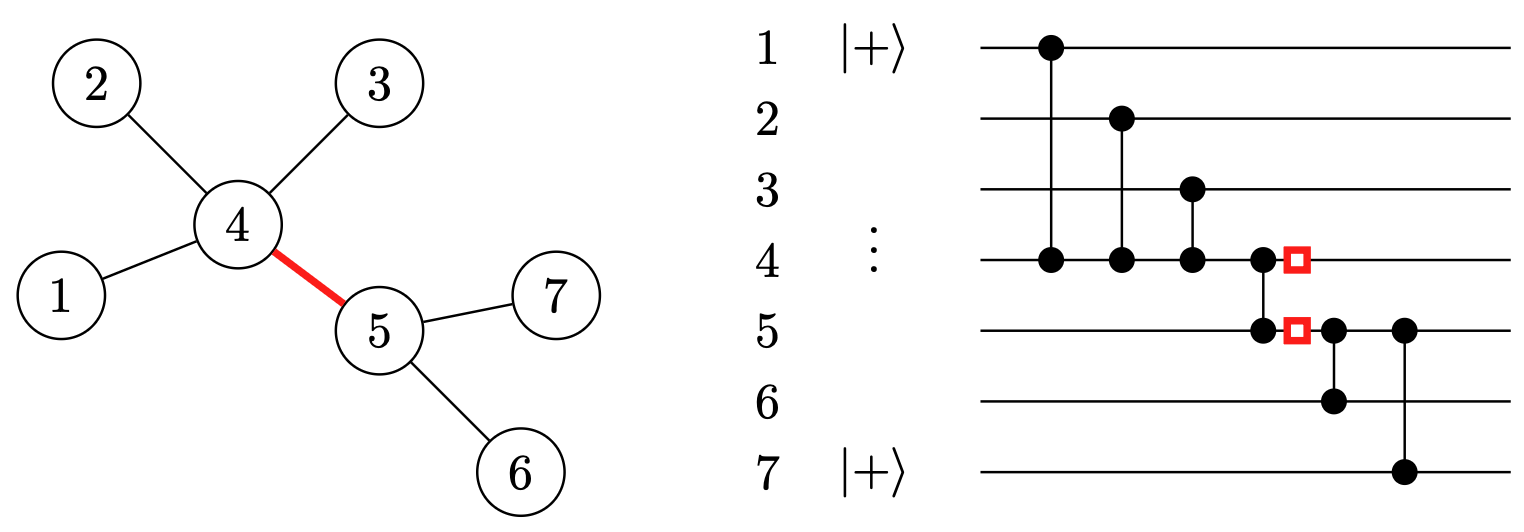
\includegraphics[scale=.32]{depolnoise.png}
\caption{An example of a single faulty entangling gate in graph state preparation. A graph state $|G\rangle$ is prepared by applying CZ gates to qubits initialized in $|+\rangle$. All CZ gates are assumed ideal except one edge $f=(4, 5)$, whose implementation is modeled as a perfect $\mathrm{CZ}_{(4,5)}$ followed by local depolarizing channels on the qubits it touches.}
	\label{fig:noisy-gate}
\end{figure}

Using the commutation relations of the \(\CZ\) gates with individual Pauli unitaries, it is easy to derive the impact of the noise happening on each qubit of a test round, recalling that all non-encoded measurement angles are then equal to 0. A \(\Z\) directly flips the measurement outcome in the \(\{\ket +, \ket - \}\) basis, while a \(\X\) has no effect on the measurement on the affect qubit, but propagates to neighboring qubits as further \(\CZ\) gates are encountered in the rest of the circuit creating \(\ket G\). This is illustrated in \cref{fig:noise-propagation}.

\begin{figure}[H]
	\centering
    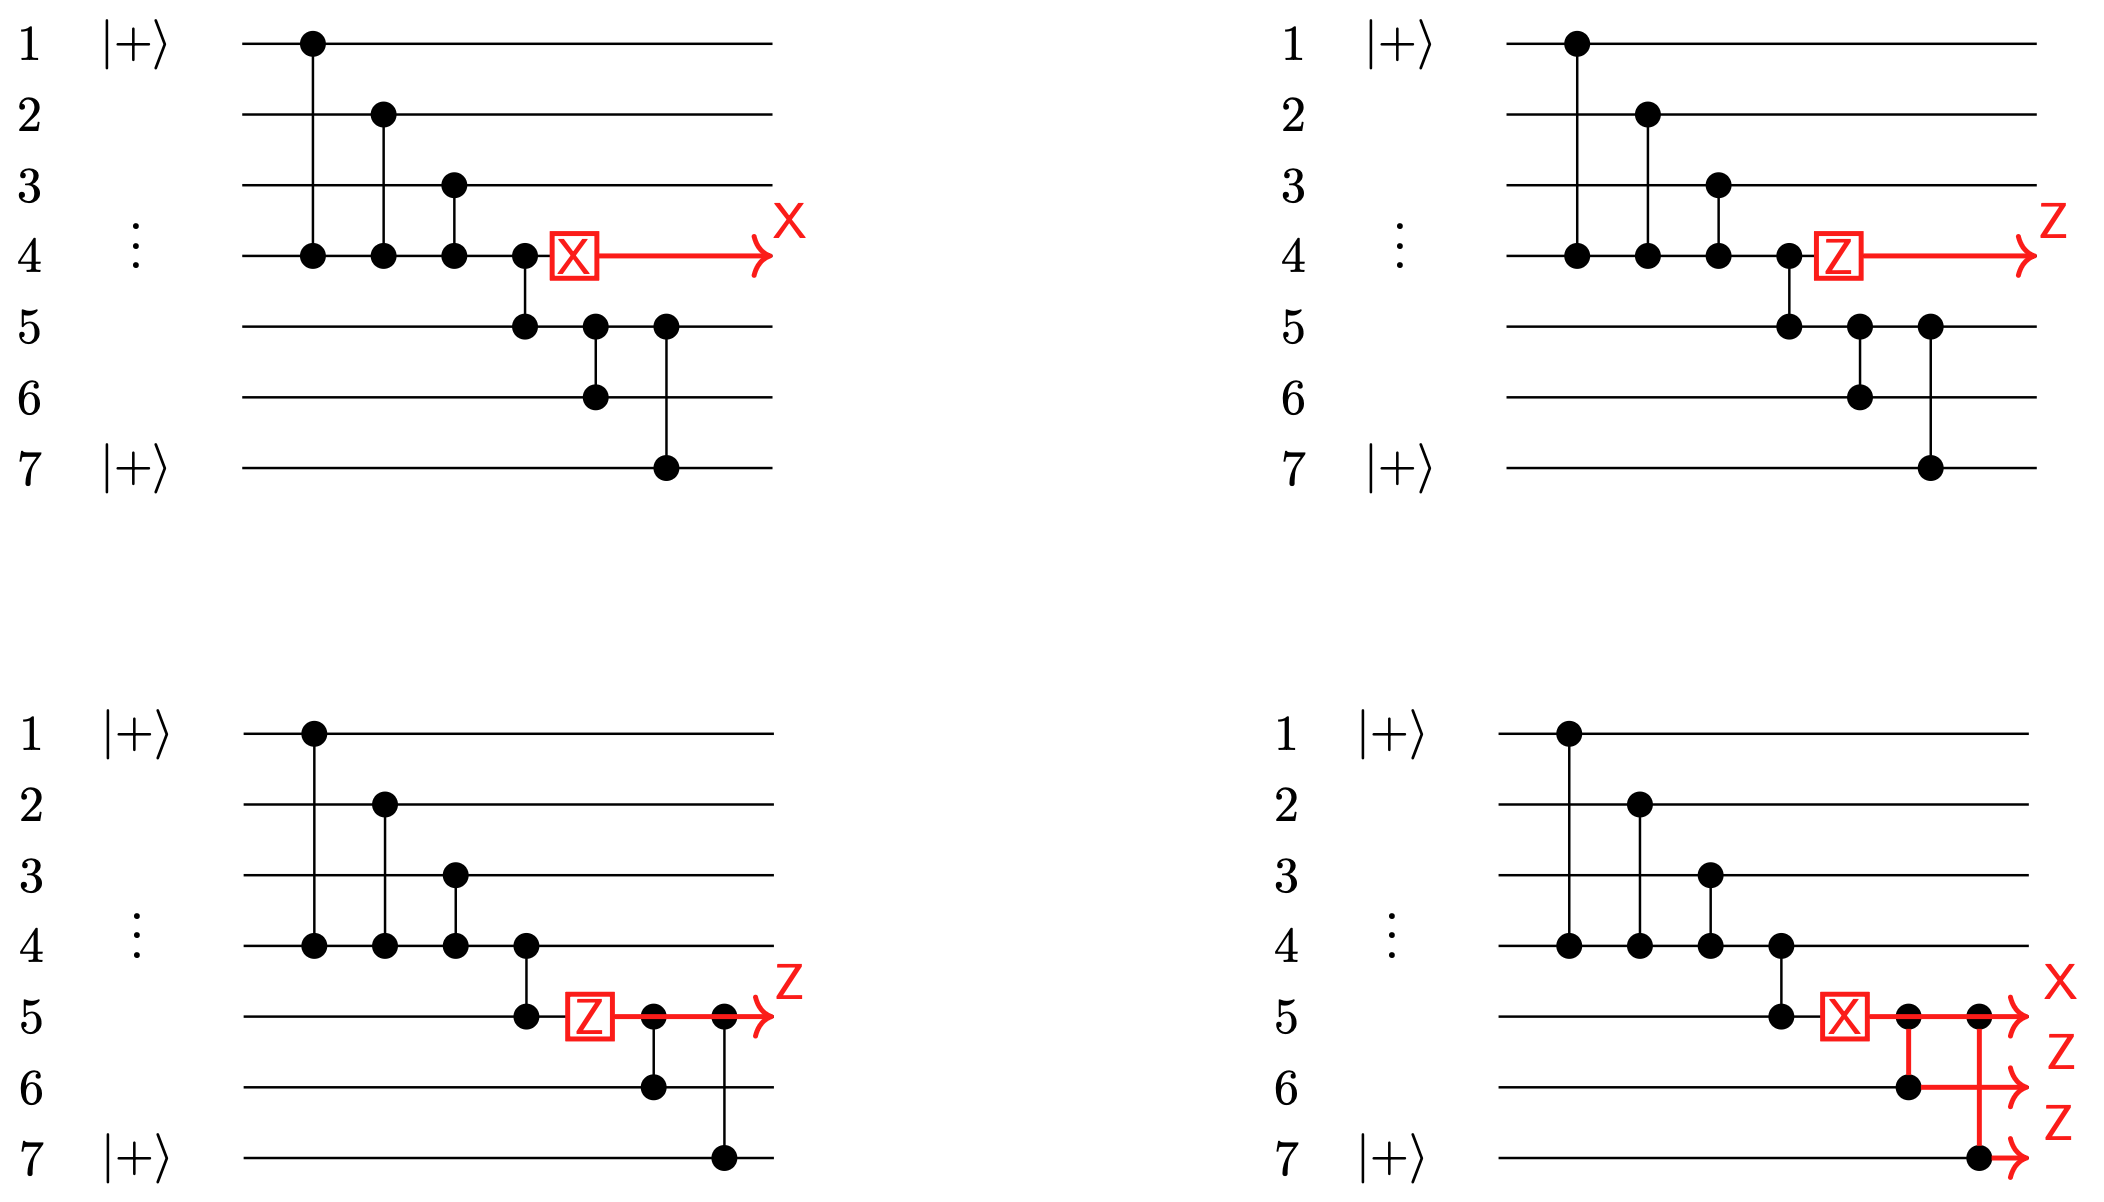
\includegraphics[scale=0.32]{propa.png}
\caption{Propagation of Pauli errors after the faulty $\CZ_{(4,5)}$ gate. The red boxed Pauli operator indicates the error immediately after the faulty gate, and each panel shows its propagation through the remaining $\CZ$ gates in the circuit. A $\X$ error on qubit $4$ (Top left). A $\Z$ error on qubit $4$ which remains localized on $4$ (Top right). A $\Z$ error on qubit $5$ which remains localized on $5$ (Bottom left). An $\X$ error on qubit $5$, which propagates forward through subsequent $\CZ$ gates,
	leaving $\Z$ errors on later neighboring qubits $6$ and $7$ while the $\X$ error remains on $5$ (Bottom right).}
	\label{fig:noise-propagation} 
\end{figure}




As a consequence, it becomes easy to identify a faulty gate by observing in rVBQC which traps are failed and which ones are not. In fact, one can notice that some traps probability are directly linked to \(\lambda_r\) and \(\lambda_s\). Using the example in \cref{fig:noisy-gate}, and the propagation of the Pauli unitaries, a bit flip for the trap in \(s\) can only happen when the depolarizing channel on qubit \(s\) yields a \(\Y\) or \(\Z\). This happens with probability \((1-\lambda_s)/2\), so that observing the failure probability of the trap in \(s\) is a direct observation of the noise happening on \(\CZ_{(r,s)}\).

Yet, for this to be possible, some information has to be communicated back to the server, as it has no access to the unencrypted data that is necessary to declare if a trap has failed or not. One could imagine that the client is well placed to perform the evaluation of the trap failure probabilities, as it is already keeping test round failures. Instead, the client could simply communicate the raw data of the test rounds, i.e., the randomness used to create the rounds comprising the encryption keys to the server and let it decrypt its measurement outcomes and estimate the failure probability directly. The important remark is that this does not affect the security of the whole scheme. As long as this transmission happens after the completion of rVBQC, the computation rounds are uncorrelated to the test rounds, and any post-processing from the server cannot create additional correlations to the computation rounds. Hence, the security is not affected by the release of the keys used for the test rounds after the protocol is completed.

This foundational example revealed two important aspects of verification:
\begin{enumerate}
\item Trap failure rate reveals information about the noise that affects the gates used to create and compute with the graph state;
\item Trap failure rate is sensitive to the order in which the noisy gates are applied as \(\X\)-noise only propagates forward in the circuit to qubits that are direct \emph{future} neighbors of the noisy one.
\end{enumerate}

\subsection{Performing ACES within rVBQC}
The previous subsection hinted at the possibility of extracting noise information from trap rounds. Yet, in order to materialize this into a concrete protocol, two gaps need to be addressed:
\begin{enumerate}
\item The relationship between the failure probability of a given trap and the noise parameters;
\item The generation of an invertible design matrix to recover individual noise parameters;
\end{enumerate}
while keeping the security of the whole protocol.

\paragraph{Trap failure probability.}
The traps in rVBQC correspond to preparations that ensure a deterministic result for an observable being measured by the server. For instance, in the simplest case, a trap at qubit \(v\) means that it is expected that for well prepared qubits, an honest server should deterministically obtain the +1 outcome when measuring the observable \(X_{v}\).\footnote{Recall that this description corresponds to the instructions that would indeed be delegated, and thus encrypted, using UBQC.} In other terms, this means that the input qubits state \(\ket{\psi(v)}\) for generating a trap at qubit \(v\) needs to satisfy:
\begin{equation}
\X\left[\cptp{C} [\ketbra{\psi(v)}] \right] = \cptp{C}[\ketbra{\psi(v)}],
\end{equation}
where \(\cptp{C} = \prod_{e\in E,\prec}\CZ_{e}\), and \(\prec\) is an ordering of $E$.

As noted in \cref{sec:test-rounds}, if one prepares the product state \(\ket{+}_v \bigotimes_{(v,w)\in E} \ket{0}_w\) as input and feeds it through the perfect circuit that generates \(\ket{G}\), it is unchanged. Now, recall that if a state is stabilized by an abelian subgroup \(S\) of the Pauli group, the projector onto that state can be written as
\begin{equation}
\frac{1}{|S|}\sum_{\cptp P\in S} \cptp P.
\end{equation}
This representation makes it straightforward to infer the output when noise affects precisely those gates that act non-trivially on the relevant stabilizers. Indeed, fix a stabilizer element \(\cptp P\in S\) and let \(C\) denote the sequence of \(\CZ\) gates chosen by the server to implement the graph state. After the noisy implementation, the contribution associated with \(\cptp P\) becomes \(\Lambda_{C}(\cptp P) \cptp P'\), where \(\cptp P'\) denotes the image of \(\cptp P\) under the ideal Clifford circuit that prepares \(\ket{G}\). It follows that the output state produced by the noisy circuit for the input state preparing a trap at \(v\) can be expressed as
\begin{equation}
\rho_{\mathrm{out}}(v) = \frac{1}{|S|} \sum_{\cptp P\in S}\Lambda_C(\cptp P)\cptp P'.
\end{equation}
Therefore, the trap failure probability satisfies
\begin{align}\label{trap_failure}
  p_{\mathrm{fail}}(v)
  & = \frac{1}{2|S|} \tr\left((\cptp I - \cptp X_v) \rho_{\mathrm{out}}(v) \right) \\
  & =\frac{1-\Lambda_{C}\left(\X_v\bigotimes_{(v,w) \in E}\Z_w\right)}{2},
\end{align}
where \(p_{\mathrm{fail}}(v)\) denotes the probability that the trap at \(v\) fails, and we used the facts that \(\tr(\cptp P)=0\) for all \(\cptp P \neq \cptp I\), while the identity contribution yields \(|S|\). In particular, the bias $P_{v}(C)$ between trap success and failure is directly given by
\begin{equation}
P_v(C) = p_{\mathrm{succ}}(v)-p_{\mathrm{fail}}(v) = \Lambda_{C} \left( \X_v \bigotimes_{(v,w) \in E} \Z_w \right).
\end{equation}	
Since traps correspond to stabilizers of the graph state, their evolution through the preparation circuit is governed by the usual conjugation rules for \(\CZ\) gates. The only degree of freedom available to the server that remains compatible with blindness is the ordering of commuting \(\CZ\) gates. Distinct orderings generally produce distinct linear constraints. Hence, by varying these orderings sufficiently, one can obtain a family of linearly independent equations that is rich enough to estimate all noise parameters \(\lambda\), provided that no intrinsic symmetry of the construction enforces unavoidable degeneracies.

% Denoting \(\tilde{\cptp{C}}\) the noisy version of the circuit \(\prod_{e\in E,\prec}\CZ_{e}\), this implies that:
% \todo[holl,inline]{Rewrite in the same way it was in the initial version.}
% \begin{align}
%   \tr(\X_v \tilde{\cptp{C}}[\ketbra{\psi(v)}])
%   & = \tr(\tilde{\cptp{C}}^{\dagger}[\X_v] \ketbra{\psi(v)}) \\
%   & = \Lambda(\tilde{\cptp{C}}^{\dagger}[\X_v]) \tr( \cptp{C}^{\dagger}[\X_v] \ketbra{\psi(v)}) \\
%   & = \Lambda(\tilde{\cptp{C}}^{\dagger}[\X_v]) \\
%   & = \Lambda(\tilde{\cptp{C}}[\W(v)]),
% \end{align}
% where \(\W(v) = \cptp{C}^{\dagger}[\X_v]\), and using the definition of \(\Lambda\) of \cref{eq:aces} together with \(\Lambda(\tilde{\cptp{C}}^{\dagger} [\X_v]) = \Lambda(\tilde{\cptp{C}} [\cptp{C}^{\dagger}[\X_v]]) = \Lambda(\tilde{\cptp{C}}[\W(v)])\).

% Now, using that the failure probability of the trap at qubit \(v\) is \(p_{\mathrm{fail}}(v) = \left (1-\tr(\X \tilde{\cptp{C}}[\ketbra{\psi(v)}])\right)/2\) we obtain:
% \begin{equation}
%   \Lambda(\tilde{\cptp{C}}[\W(v)]) = 1 - 2 p_{\mathrm{fail}}(v),
% \end{equation}
% or alternatively, 
% \begin{equation}
%   \Lambda(\tilde{\cptp{C}}[\W(v)]) = p_{\mathrm{succ}}(v) - p_{\mathrm{fail}}(v),
% \end{equation}
% where \(p_{\mathrm{succ}}(v)\) denotes the success probability for the trap at qubit \(v\). As noted before, the structure of rVBQC allows for the client to transmit all the randomness used for the trap rounds after the completion of the protocol, so that the server can evaluate \(p_{\mathrm{succ}}\) and \(p_{\mathrm{fail}}\) for each \(v \in V\), without comprimising the security of the protocol.

\paragraph{Generating an invertible design matrix.}
While the previous paragraph demonstrated that rVBQC allows to perform one crucial step of ACES evaluation of some \(\Lambda\)'s, to complete the extraction of noise model parameters, it is necessary to invert the relationship between the gate-level noise model, i.e.,~\(\lambda_{e}\), and the circuit-level noise model, i.e.,~\(\Lambda\), see \cref{eq:aces}. When ACES is applied in a stand-alone fashion, this is usually done by varying the circuit applied and the input states. Yet, in the scenario described here, there is no such freedom. The reason is that the circuit \emph{must} implement the Clifford \(\cptp{C}\) that creates the graph state \(\ket G\) from \(\ket{+}^{|V|}\) states. The reason is that rVBQC imposes the structure of test rounds containing the traps. Adding extra rounds designed solely for noise estimation purposes is always possible, but they wouldn't correspond to recycling data from rVBQC itself.

Hence, the question of generating an invertible generating matrix should be considered with the additional constraint imposed by rVBQC, that is, with a fixed target Clifford \(\cptp{C}\) and using \(\X\) measurements only, so that these correspond to data generated by rVBQC traps.  Recalling \cref{eq:aces} and the example of \cref{fig:noisy-gate} and \cref{fig:noise-propagation}, we see that one possibility is to change the order of the \(\CZ\) gates that implement \(\cptp{C}\). While for any permutation \(\sigma: E \rightarrow E\) we have,

\begin{equation}
\cptp{C} = \prod_{e \in E, \prec} \CZ_e = \prod_{e \in E, \prec} \CZ_{\sigma(e)}, 
\end{equation}
where \(\prec\) is an order over \(E\), their corresponding noisy versions, respectively defined as \(\tilde{\cptp{C}}\) and \(\tilde{\cptp{C}}_{\sigma}\) do not match. This is because, as noted before, noise propagates to future neighbors, which depends on the order in which \(\CZ\) gates are applied. By choosing various permutations \(\sigma \in \Omega\), where \(\Omega\) is a subset of the permutations of \(|E|\), it then becomes possible to generate a different equation linking the observed probabilities of success and failures of a trap at a given qubit \(v\) given the chosen \(\sigma\). Using this freedom, ACES is integrated into rVBQC in the following way:
\begin{protocol}[rVBQC with ACES]
  \label{proto:vbqc-aces}
\item
  \begin{algorithmic}[0]
    \Procedure{Server Initialization}{}
    \State The server chooses randomly a permutation \(\sigma_i \in \Omega\) for each \(i \in [N]\).
    \EndProcedure
    
    \Procedure{rVBQC Execution}{}
    \State The Client and the server perform rVBQC, where the server applies the \(\CZ\) gates in the order defined by \(\sigma_i\) for round \(i\).
    \EndProcedure
    
    \Procedure{Randomness Sharing}{}
    \State The client sends all the randomness used during the test rounds to the server.
    \EndProcedure
    
    \Procedure{ACES}{}
    \State The server computes the success and failure probabilities for each trap \(v\) and each order \(\sigma\), and inverts the corresponding design matrix to recover the gate-level noise parameters.
    \EndProcedure
  \end{algorithmic}
\end{protocol}

Note that in addition to the order of \(\CZ\) gates, one could perform other changes that still implement the same unitary \(\cptp{C}\), while increasing the capability to generate more equations linking observed success and failure probabilities for traps and gate-level noise parameters. For instance, one could replace any \(\CZ\) gate by an odd number of the same \(\CZ\) gate, and apply shifts on top of this. We will comment on this ability at the end of the next section. This remark nonetheless outlines the important remaining question, whether one can estimate noise parameters for a reasonably complex model in spite of the very restricted sets of circuits and measurements that are compatible with the security of rVBQC. We will answer this question by instantiating rVBQC with ACES for a specific noise model in the next section. The reason for not seeking a theoretical answer for it is that for ACES alone, i.e.,~without rVBQC, the answer will indeed be strongly dependent on the noise model. As the number of parameters to estimate increases, the task becomes more complex, and more equations need to be generated. For purposefully complex noise models, ACES can become intractable, while for reasonable noise models, it is generally not the case.


